%\section{Method}
\section{Backgrounds}

First of all, we introduce basic physics of the lightning and explain details of the dielectric breakdown model~\cite{Niemeyer1984} that is widely used for simulation of the lightning. Then, we present details of our method that quickly generates the lightning shape and renders the lightning with glow effect.



\subsection{The Physics of Lightning}

Lightning occurs when a large charge difference exists between two area such
as cloud and ground. 90 percent of all cloud-to-ground lightning is
\textit{downward negative lightning} that starts from negative charges
under the cloud and spreading out to positive charges on the ground. Negative
charges move to the ground through the lightning stream for the earth and air
to reach the equilibrium state.

Lightning strikes the ground through several steps. The first stroke is called
\textit{stepped leader} where negative charges spread out and hit the ground
firstly through points that have less residual resistance in the air. When the
stepped leader reaches the ground, positive charges on the ground move up to
the cloud rapidly following the path of the leader with a strong flash and
sound. It is called \textit{return stroke}. After the return stroke, subsequent
strokes, \textit{dart leader}, may appear the following the path of the
previous leader when enough charges remain between the cloud and ground.
%. It is called \textit{dart leader}.
Several times of return strokes and dart leaders appear after the first stepped
leader during a very short period. The stepped leader has many branches. On the
contrary, dart leader has fewer branches and is a little darker than the
stepped leader.

According to observations, lightning branches maintain an angle of about 16
degrees with their parent branch, and the lightning shape has a fractal
dimension of approximately 1.7~\cite{Niemeyer1984} like other natural phenomena
such as ice crystal, lichen, and so on. All the patterns that have this fractal
property are known as ~\textit{Laplacian growth}~\cite{Hastings1998}.




\subsection{Dielectric Breakdown Model (DBM)}


\begin{figure}[t]
	\centering
	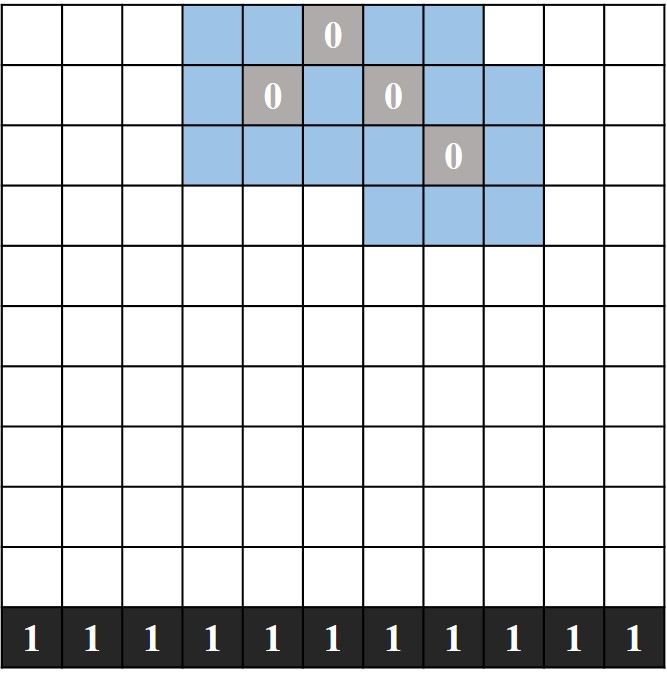
\includegraphics[width=2.0in]{fig/dbm_grid}
	\caption{Grid representation of DBM for the lightning. Black and grey
cells represent  the positive charges on the ground and the negative charges at
the bottom of cloud, respectively. Blue cells are the candidates for the next
advance. }
	\label{fig_dbm_grid}
\end{figure}

DBM~\cite{Niemeyer1984} uses a regular grid representation and calculates an
electric potential, $\phi$, for each grid cell to simulate the dielectric
breakdown
phenomenon. Figure~\ref{fig_dbm_grid} shows a grid representation for the
lightning simulation. Negative charges are placed at the top and their electric
potentials are set to $\phi=0$. While, positive charges are placed at the
bottom and they
set to $\phi=1$. The boundaries of the grid are also set to $\phi=0$. These
three type of electric potentials are fixed and treated as boundary conditions.
For the remaining grid cells, the electric potentials are calculated by solving
the Laplace equation with the boundary condition:
\begin{equation} \label{eq_laplace}
\bigtriangledown^2\phi = 0
\end{equation}

After computing the electric potential of the overall grid, the subsequent
growth of the lightning is selected randomly according to the electric
potential as a probability among candidate cells that are neighboring to
the cells of
the lightning. In Figure~\ref{fig_dbm_grid}, blue cells are the candidate cells
given the current lightning pattern. The probability of each candidate cell $i$
is computed as the following:
\begin{equation} \label{eq_prob}
P_{i} = \frac{(\phi_{i})^\eta}{\sum_{j=1}^{n} (\phi_{j})^\eta},
\end{equation}
 %~\ref{eq_prob}. 
where 
%\textit{i} and 
\textit{j} is an index of each candidate cell and \textit{n} is the  total
number of the candidate cells.

The electric potential for the chosen cell is then set to $\phi=0$. The chosen
cell becomes the new cell of the lightning shape and is added into a new
boundary condition.  This process is repeated until the lightning reaches the
cells that have the positive charge on the ground. Figure~\ref{fig_dbm_process}
shows overall process of generating the lightning shape by DBM. $\eta$ can
control the number of branches. As $\eta$ increases, the lightning shape has
fewer sub-branches. Therefore, it is often called $\eta$ model. A value of two
or three is used for a realistic lightning.

\begin{figure}[t]
	\centering
	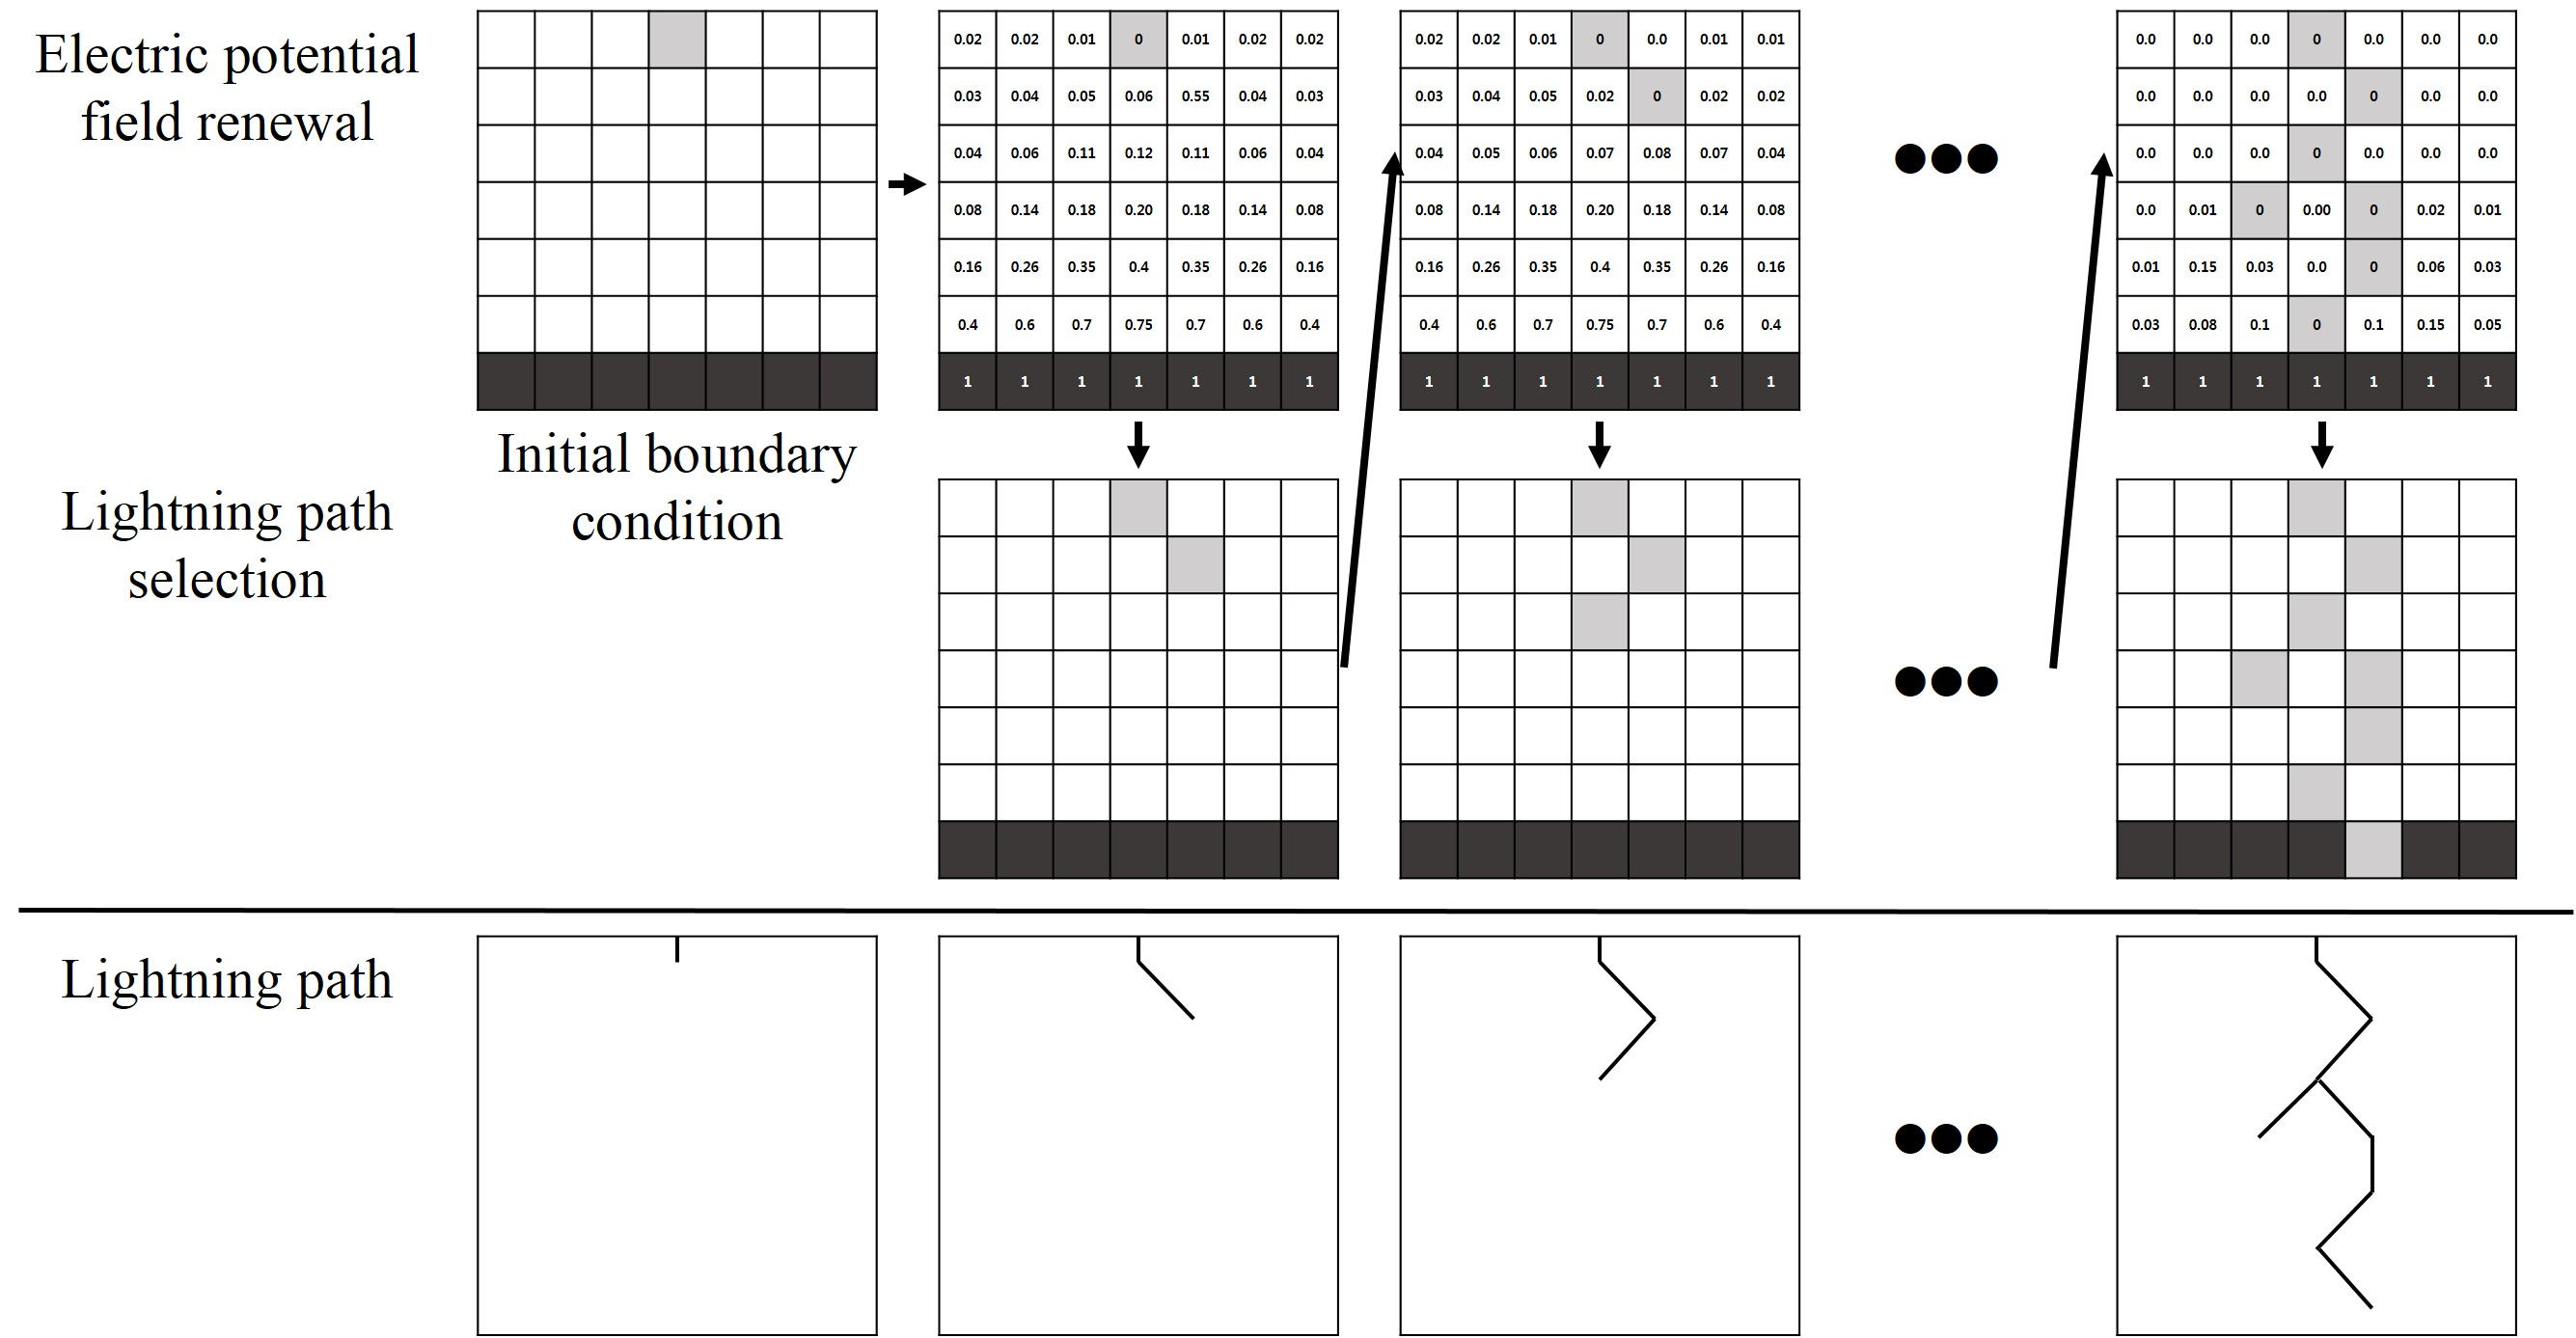
\includegraphics[width=3.2in]{fig/dbm_process}
	\caption{\YOON{Use a high resolution image or vector rep.}The process of generating the lightning shape by DBM.}
	\label{fig_dbm_process}
\end{figure}




%methods proposed by 

Kim and Lin~\shortcite{Kim2004,Kim2007} proposed practical techniques to
realize DBM for generating the realistic shape of the lightning.
% They use the
%~\textit{Dielectric Breakdown Model}, which is based on 
These techniques are based on DBM and
%physics and 
solve the
Laplace equation 
%to get the electric potential of each grid cell 
by using the conjugate gradient method with a diagonal preconditioner. 
%However,
While this technique is based on DBM and can generate realistic shapes,
it can take a high computational time,
% to generate the lightning shape 
because the conjugate gradient method 
has a time complexity $O(G^{1.5})$~\cite{Shewchuk1994}, where \textit{G} is the number of the grid
cells.
%. The time complexity for selecting new advance of the lightning is $O(g)$
%and ~\textit{g} is the number of the candidate cells. 
We found that it takes about 1.5 seconds to create the lightning shape by using
128 x 128 grid map on our tested machine.
%a typical
%personal computer. It can not be suitable for the real-time application like
%games even if it can make a realistic shape.

\YOON{How about ted's laplacian paper?}



%%%%%%%%%
\Skip{

is an iterative algorithm that reduces
error value until it converges to
target. Two processes are repeated to create the form of lightning. First one
is a renewal of the electric potential by solving the Laplace equation. Another
one is selecting next growth cell of the lightning among the candidate cells.
The time complexity of calculating the electric potential is
$O(G^{1.5})$~\cite{Shewchuk1994} and ~\textit{G} is the number of the grid
cell. The time complexity for selecting new advance of the lightning is $O(g)$
and ~\textit{g} is the number of the candidate cells. It takes about 1.5
seconds to create the lightning shape by using 128 x 128 grid map on a typical
personal computer. It can not be suitable for the real-time application like
games even if it can make a realistic shape.
}
%%%%%%%%%%%%%%%%%%%%


\section{Our Method} 


%\subsection{Generating a Lightning Shape}
%\subsection{Generating a Lightning Shape}
\subsection{Approximate Potential Method}

We propose a method that approximates important trends of electric potentials
of the candidate cells quickly for interactive applications. We do not solve
the Laplace equation using numerical solutions like the conjugate gradient
method.
%. It takes
%too much time for a request of the real-time manner. 
Instead, we approximate electric potentials by considering characteristics of
the value distribution on the electric potential field.

We found that there are simple properties for the electric potential field
according to three types of cells:
\begin{itemize}
%$\bullet$ 
\item The electric potential increases toward the positive charge cells.
%$\bullet$ 
\item The electric potential decreases toward the negative charge cells of the
lightning path.
%$\bullet$ 
\item The electric potential decreases toward the boundary.
	%\label{list_obs}
\end{itemize}
	
\begin{figure}[t]
	\centering
	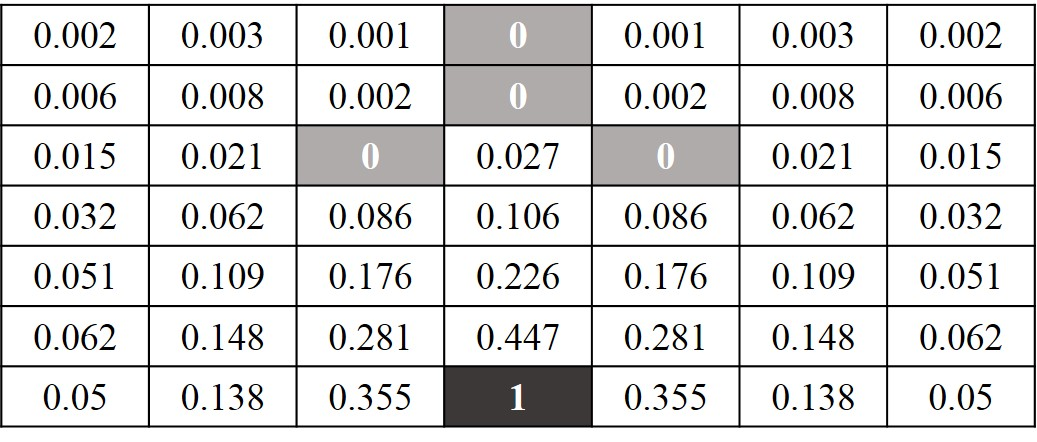
\includegraphics[width=3.0in]{fig/cgm_value_distribution}
	\caption{
This shows values of the electric potential field after solving the Laplace
equation using the conjugate gradient method on the 7 x 7 grid map.}
	\label{fig_cgm_value_distribution}
\end{figure}



Figure~\ref{fig_cgm_value_distribution} shows the result of electric potentials
on a 7 x 7 grid map after solving the Laplace equation. The electric potential
depends on distances to three types of cells like other physical
equations for the electrostatics such as Coulomb's law\YOON{Give a citation on a physics book for this}. 

In fact, we are not the first one to observe such phenomenon.  In physics, it
is well known that a potential at a point $x$ under the Laplace equation is
equal to the average potential computed on a virtual sphere located at the
point $x$, each of which is governed by the electric potential equation\YOON{cite: 
Introduction to Electrodynamics, Third Edition, David J. Griffiths}:
%(Eqn.~\ref{eq_ep})
\begin{equation} 
V = 
%	\sum_{i=1}^{n}
%	\frac{1}{4\pi\epsilon_{0}}(\frac{q_{i}}{r_{i}}),
	\frac{1}{4\pi\epsilon_{0}}(\frac{q}{r}),
	\label{eq_ep}
\end{equation}
where 
%\textit{n} is the total number of charges, and 
\textit{q} and \textit{r} are an electric point charge and the distance from
the charge to the point $x$, respectively.  This idea is also adopted by the
works of Sosobaram et al.~\cite{Sosobaram2001} and Kim et al.~\cite{}\YOON{Cite
the ted kim work here}, while Kim el al. used the spherical coordinate.
%the electric potential equation is used for
%selecting a next path of simulating the lightning shape~\cite{Sosorbaram2001}:


We also found that these techniques, unfortunately, are less robust to generate interesting branching patterns of the lighting shape.
This is mainly because
%Distance(~\textit{r}) is an important value.
%However, the results of Eqn.~\ref{eq_ep} 
the electric potential equation gives very similar values between the candidate
cells and other charges in the boundary condition.
As a result, 
those candidate cells are likely  to have  similar probabilities of being chosen for the 
subsequent growth of the lightning path. 
%of selecting 
%Because the candidate cells are the
%neighboring cells to the current lightning path and have a similar distance to
%the negative charge cells of the lightning path and the positive charge cells.
The computed final lightning shape, thus, tend to spread out to all directions
from the starting position due to the similar probability. 

%Also, it can not show the property for
%the boundary because there are no parameters for the boundary in
%Eqn.~\ref{eq_ep}.



%constant part and assume that the charges have the same amount. 
Instead, we propose to use a simple approximation that has the same trend of
$1/r$ to the electric potential equation, but is controlled by $\rho$ as the
following:
% on
%distance computation:
%$\rho$ is a
%scaling coefficient for an influence of the distance.
\begin{equation} \label{eq_our_ep}
V_{appro} = \sum_{i=1}^{n}(\frac{1}{r_{i}})^{\rho},
\end{equation}
%It is controlled by the $\rho$ in our
%method, and
where $\rho > 1$.
% it must be greater than 1. In addition to that, we can manage the
%number of branches of the lightning shape by $\rho$ like $\eta$ of the DBM. 
As the value of $\rho$ increases, the lightning shape has fewer branches and
show stronger directionality to the target position. Figure~\ref{fig_comp_rho}
shows lightning shapes with different $\rho$ values.

\begin{figure}[t]
	\centering
	\subfigure[$\rho = 2$]{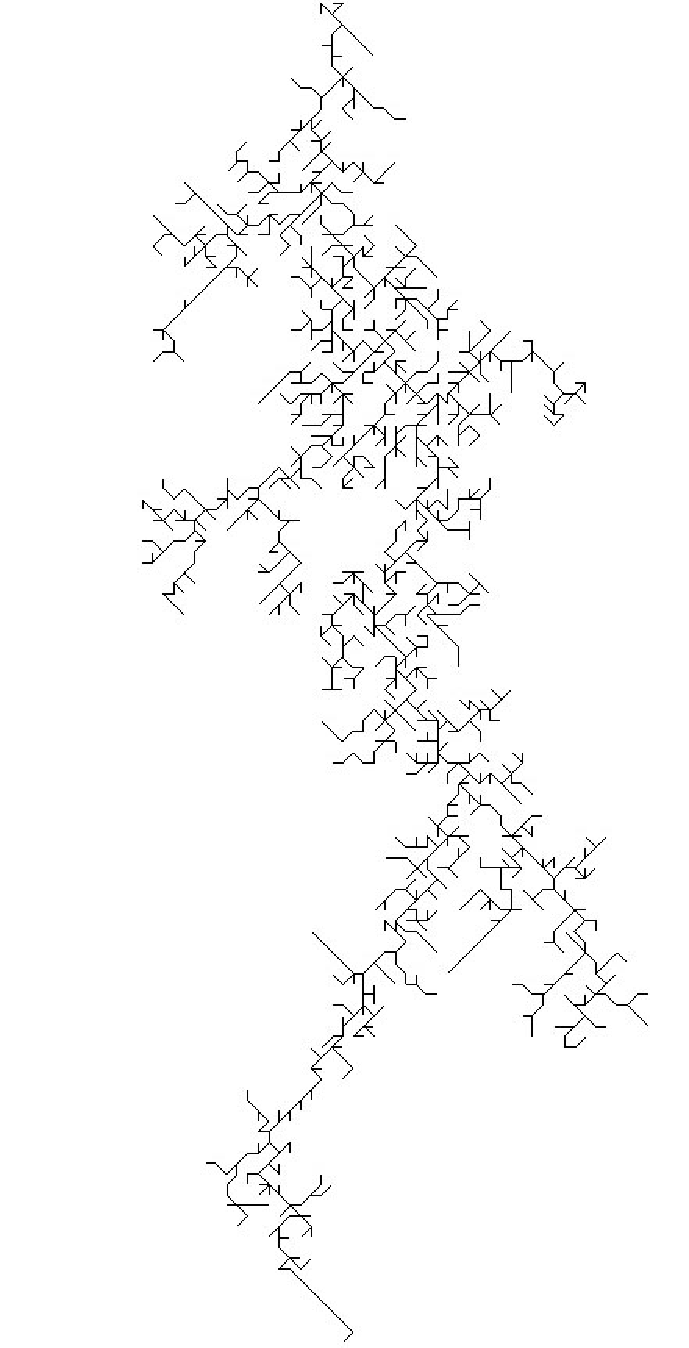
\includegraphics[width=1in]{fig/our_128_rho2}}
	\subfigure[$\rho = 3$]{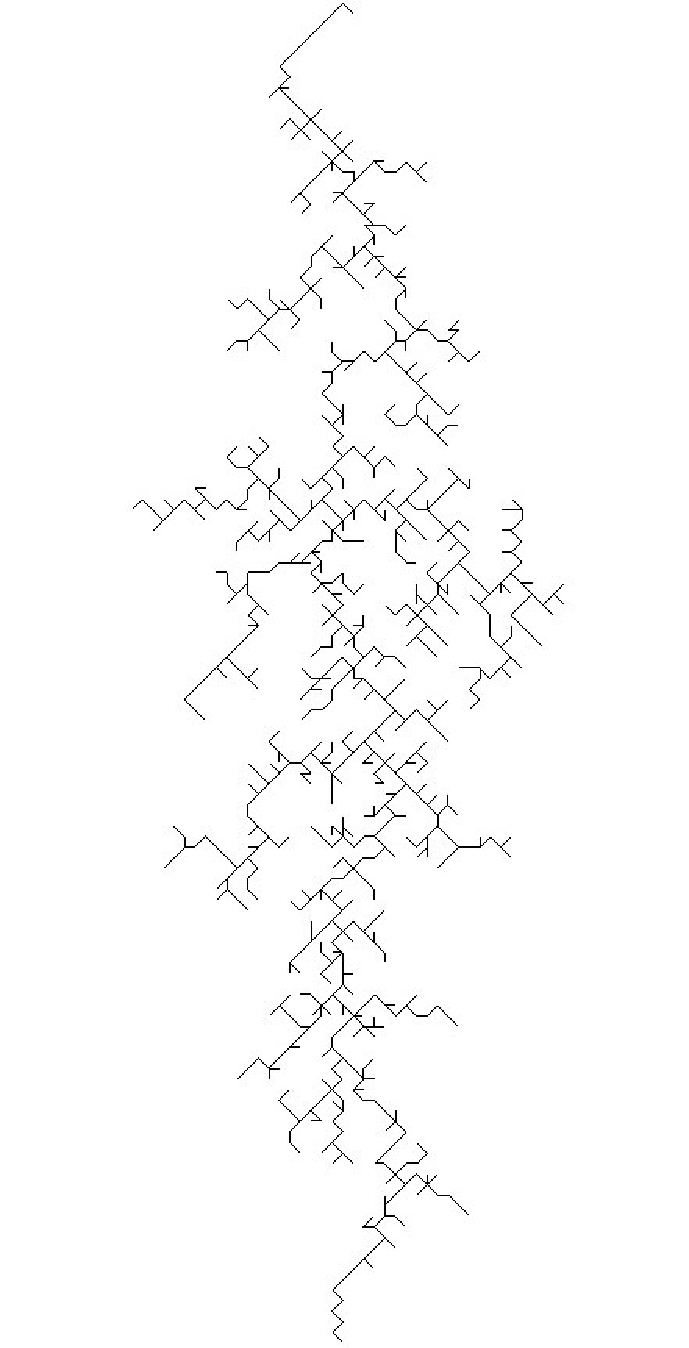
\includegraphics[width=1in]{fig/our_128_rho3}}
	\subfigure[$\rho = 4$]{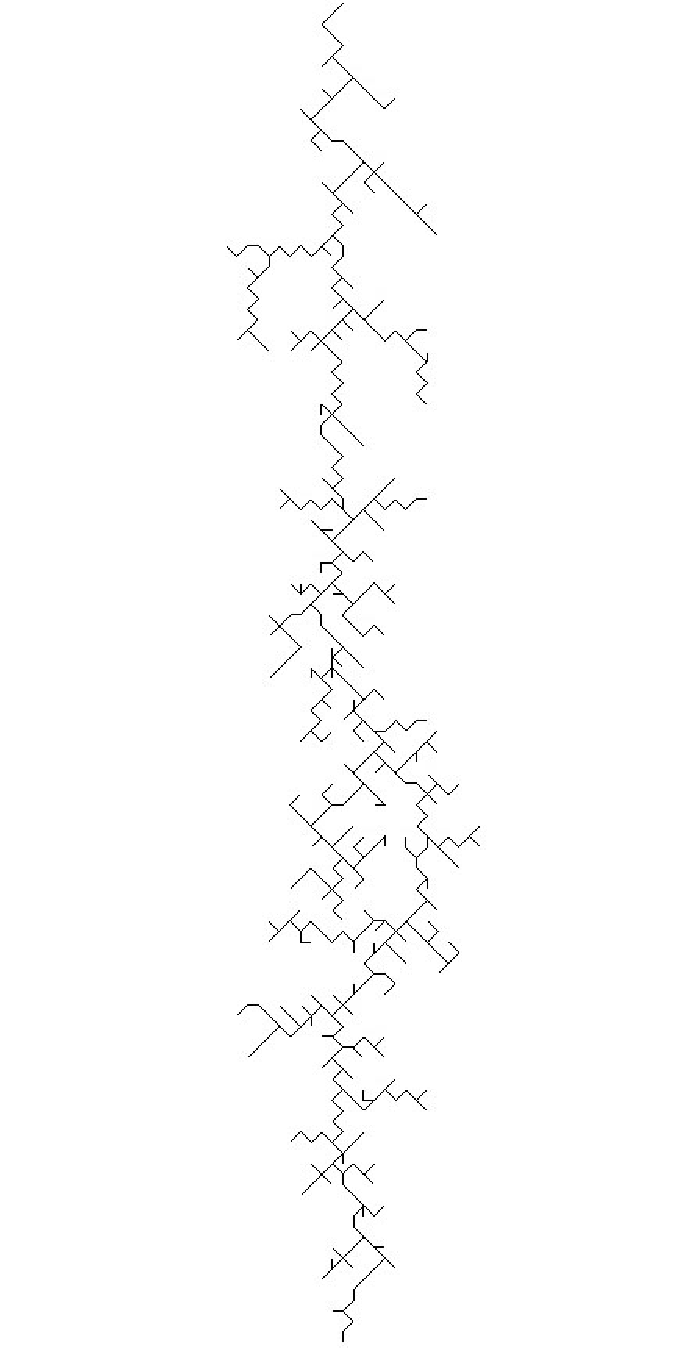
\includegraphics[width=1in]{fig/our_128_rho4}}
	\caption{Lightning shapes as a function of $\rho$.}
	\label{fig_comp_rho}
\end{figure}



\YOON{can you show benefits of rho over the prior methods given the etah term?}

We then divide the charges into three types of positive charges, negative
charges of the lightning path, and boundary charges, and calculate the electric
potentials separately into \textit{P}, \textit{N}, and \textit{B},
respectively,  with our approximate equation Eqn.~\ref{eq_our_ep}.  


\begin{figure}[t]
	\centering
	\subfigure[CGM]{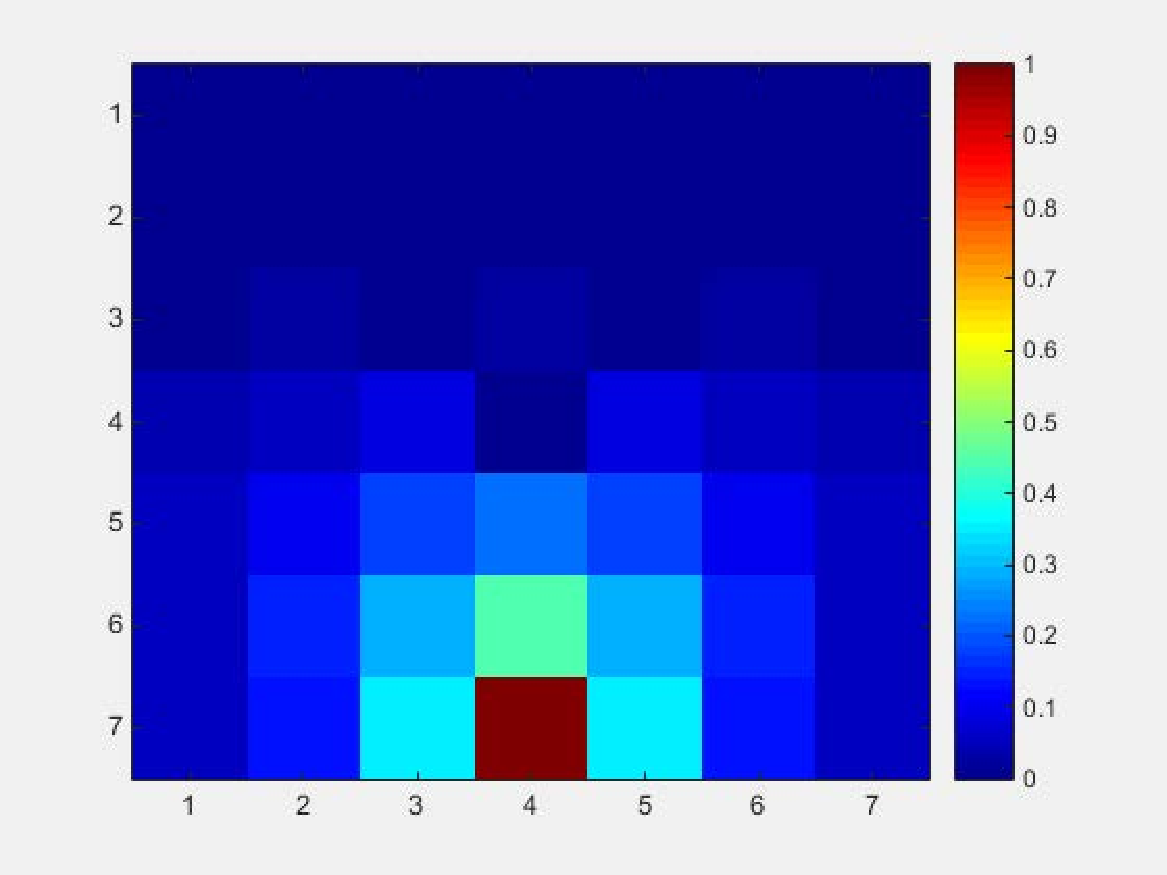
\includegraphics[width=1.6in]{fig/simple_7_cgm}}
	\subfigure[Our method ($\rho=2$)]{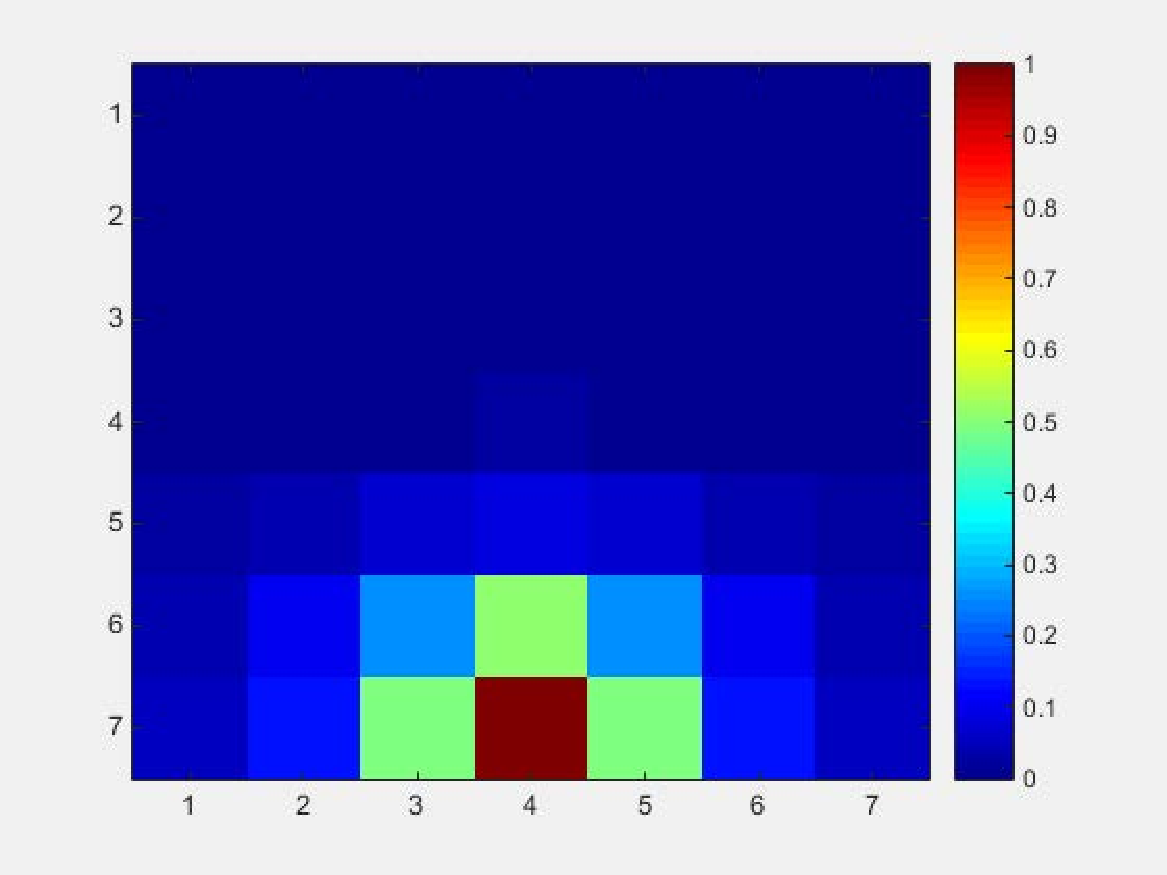
\includegraphics[width=1.6in]{fig/simple_7_our}}
	\caption{Heat map visualization for the result of electric potential
	fields after the normalization.  They show similar trends given the
	electric potential trends related to positive, negative, and boundary
	cells.
%	mentioned in \ref{list_obs}. 
	%Left is a result that is solved by the conjugated gradient method.
	%Right is a normalized result solved by our method.
	}
	\label{fig_comp_heatmap}
\end{figure}


Ideally, we
need to sum those three terms with \textit{P}, \textit{N}, and \textit{B}
  to compute the final potential according to the electric potential function. 
We however found that simply summing them does not create interesting branching
patterns.  For example, consider `tip effect' indicating a region surrounded by
negative charges has a high probability to have the negative
charge~\cite{Niemeyer1984}.  However, we found that the summation such terms
fail to produce the effect.  This issue arises mainly because we compute
potentials by assuming each charged point in the center of  a cell and thus the
term of $1/r$ cannot create extremely small values between even neighboring
cells.

%And then, we multiply them to maximize the difference among the candidate cells
%and get the final electric potential(Eqn.~\ref{eq_fianl_ep}). ~\textit{P},
%~\textit{N}, and ~\textit{B} are calculated results by Eqn.~\ref{eq_our_ep} for
%positive charges, negative charges of the lightning path, and boundary charges
%respectively. The electric potential is proportional to ~\textit{P} and
%inversely proportional to ~\textit{N} and ~\textit{B}.

To address this issue, we propose to use the following simple function: 
\begin{equation} \label{eq_fianl_ep}
\phi = \frac{P}{N \times B}.
\end{equation}
Since we divide potentials of positive charges with those of negative ones,
we can assign stronger negative energy among nearby negative charges.

Heat map visualization of electric potential fields that are computed by the
conjugate gradient method and our method are shown in
Figure~\ref{fig_comp_heatmap}. 
%We normalized the electric potential from 0 to
%0.5 because the result of our method can have more than 1. 
%In
%Figure.~\ref{fig_comp_heatmap}, 
We can visually see that these two graphs show similar value distributions.


\subsection{Clustered Potentials}
%\YOON{This should be in a separate section.} 

\YOON{Start from here....}


Our method calculates the electric potential only for the candidate cells, not
for all the cells on the grid. 
For the boundary charges, it is a static value for
the scene. So it can be pre-computed and loaded while loading the scene data.
We don't need to compute this value for every process for the renewal of
electric potential. Start and target positions of the lightning can be set at
initializing step. For the positive charges, we need a one-time computation and
then can reuse it. Our method can generate the lightning shape quickly thanks
to these reasons. For the negative charges, however, as the number of the
lightning branches increases, the number of the lightning charge and candidate
cells for the next growth increases. Computation time for the negative charges
increases linearly. 

To reduce the computation time for the negative charges, we
utilize a clustering technique. Negative charges that are near to a candidate
cell affect more than negative charges that are far away. We divide grid cell
to more coarse level and calculate a representative charge that has an average
position and scaled amount of negative charges in the same cluster. If the
negative charges are in the same cluster to candidate cell, we use
Eqn.~\ref{eq_our_ep} for each of the negative charges directly. Otherwise, we
compute the electric potential with one representative charge that has scaled
amount.
Figure.~\ref{fig_cluster_grid_map} shows the clustered grid map with representative charges and how to compute the electric potential for the negative charges.

\begin{figure}[t]
	\centering
	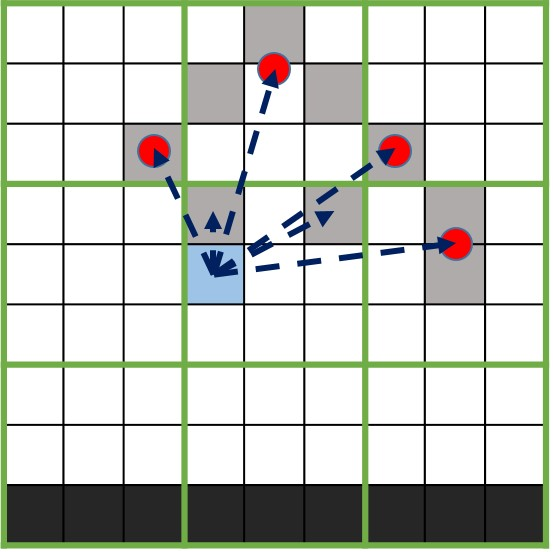
\includegraphics[width=2.0in]{fig/cluster_grid_map}
	\caption{Clustered grid map with representative negative charges to compute the electric potential for the negative charges. The 3 x 3 grid of green color is clustered grid map, and red circles are the representative charges in each cluster. Grey and black cells represent the negative charges of the lightning path and positive charges, respectively. Blue cell is one of the candidate cells. It calculates the distance for four representative charges which are not in the same cluster and two negative charges which are in the same cluster.}
	\label{fig_cluster_grid_map}
\end{figure}


%%%%%%%%%%%%%%%%%
\Skip{
We multiplied P, N, and B to maximize an influence for computing the electric
potential for the candidate cells. But, one for $\rho$ is not enough because
the candidate cells have a similar position. We also need to emphasize the each
of them to maximize the difference. 
}
%%%%%%%%%%%%%%%%%%


Figure~\ref{fig_comp_lightning_shape} shows the lightning shapes that are
generated by ~\cite{Kim2004} and our method on 128 x 128 grid map. Our methods
can make the lightning shape which is visually similar to the result produced
by the physically based approach.\JS{Do we need to add fractal dimension for
both of them?}

\begin{figure}[h]
	\centering
	\subfigure[Result by CGM]{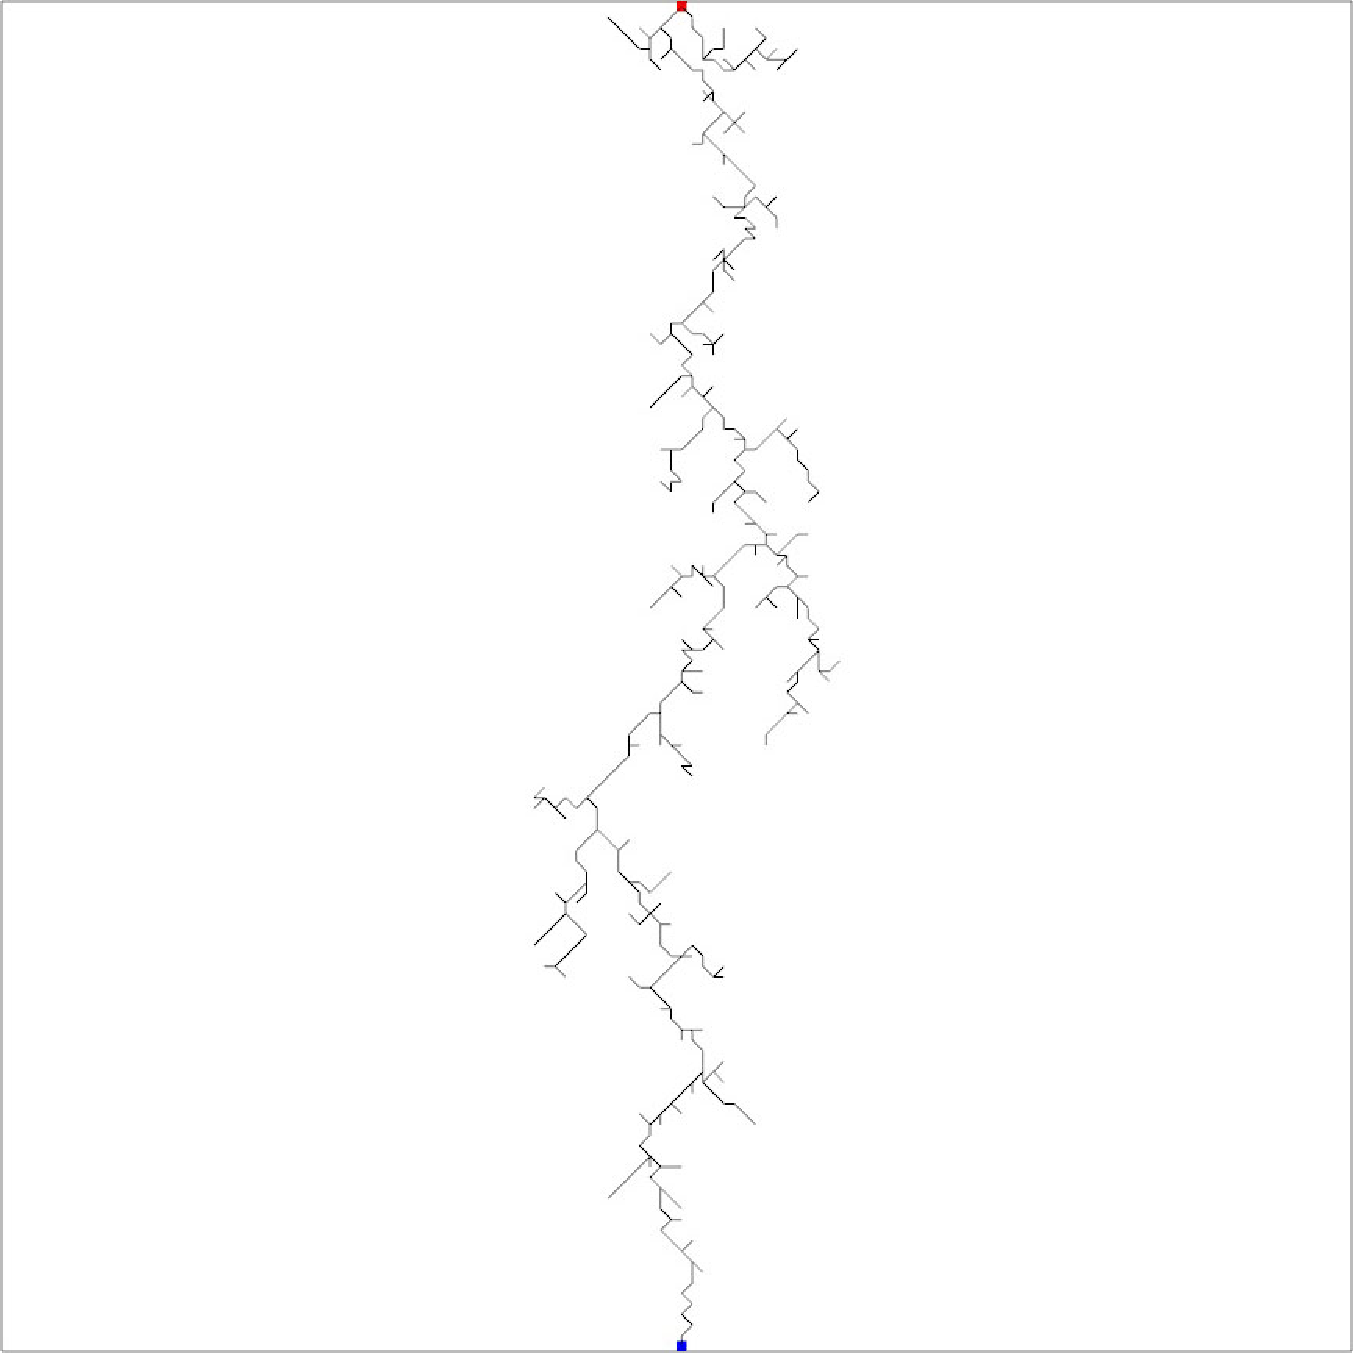
\includegraphics[width=1.6in]{fig/kim_128}}
	\subfigure[Result by our method]{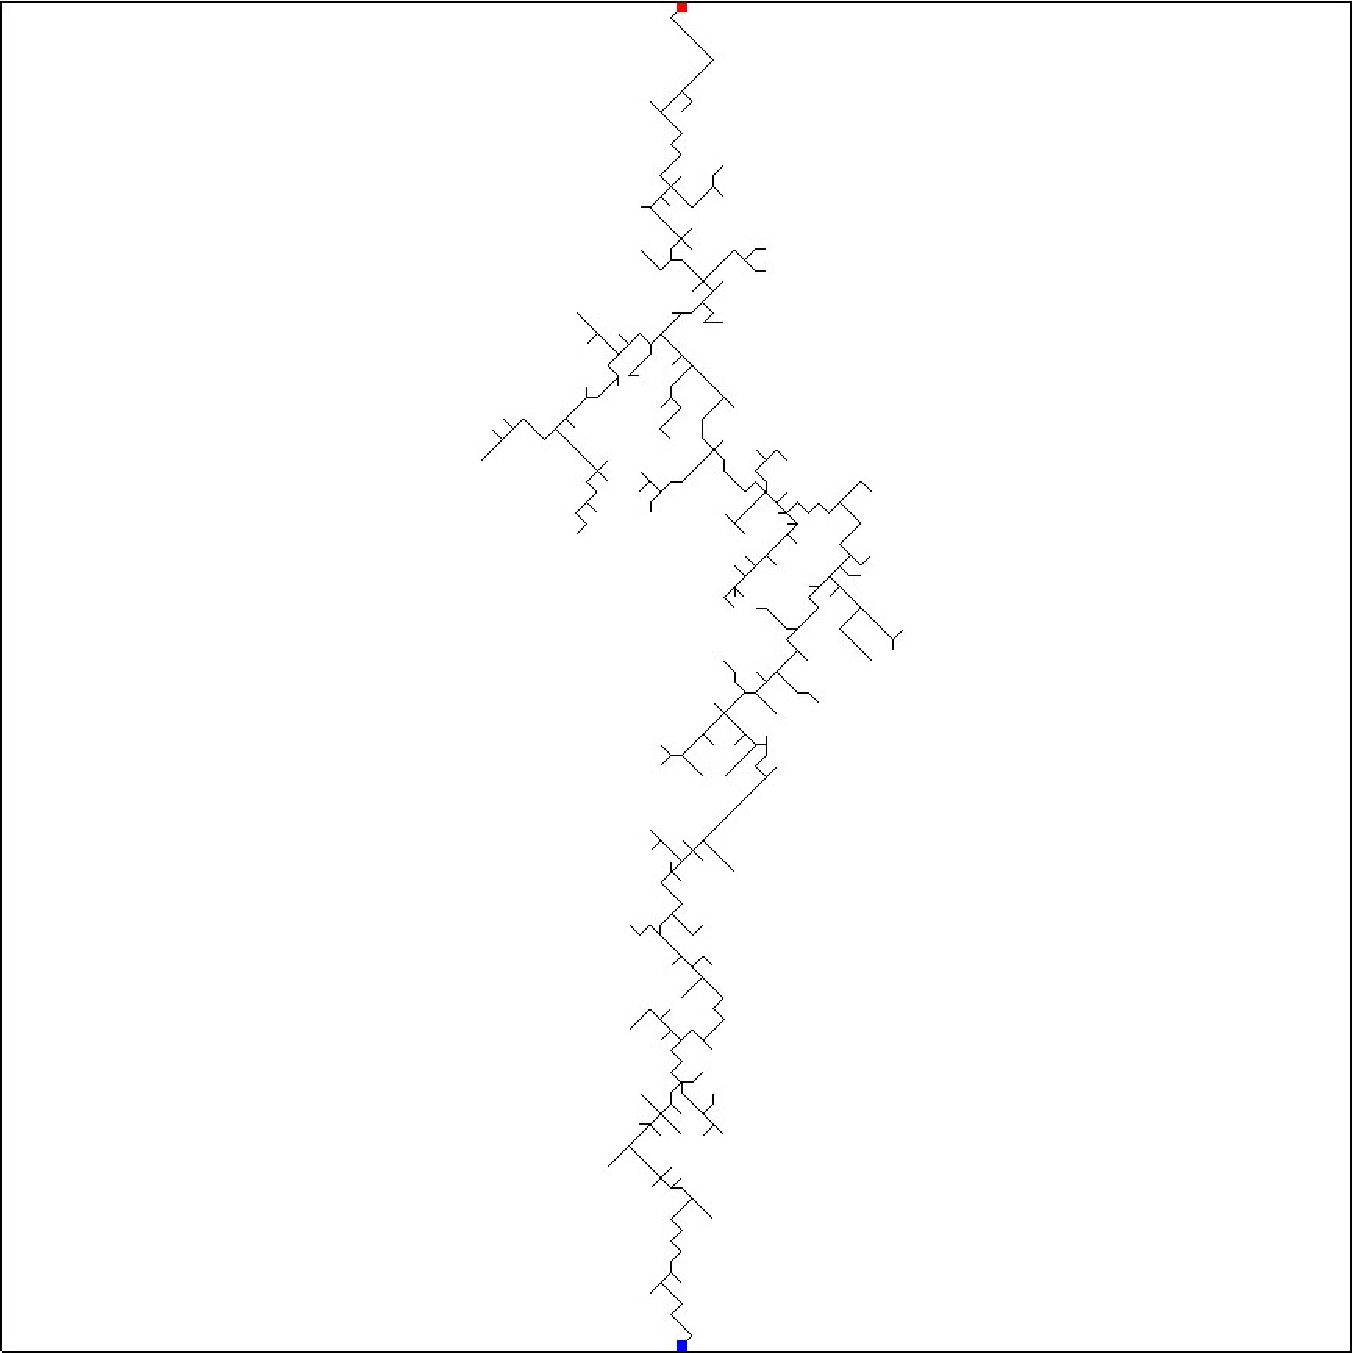
\includegraphics[width=1.6in]{fig/our_128}}
	\caption{The comparison of the lightning shapes. Red and blue rectangles represent the starting and goal position of the ligntning. Left is the result by Kim and Lin and Right is the result by our method.}
	\label{fig_comp_lightning_shape}
\end{figure}



\subsection{Considering Obstacles}

There can be many obstacles that should not be hit by the lightning such as buildings in the game scene. Of course, we can make the lightning hit the obstacles, if we want, by setting the positive charges on them. However, we need to consider the obstacles if we want that the lightning avoids them. For the obstacles, it is the same approach to the boundary. So, the final result can be computed by Eqn.~\ref{eq_fianl_ep_with_obs} for the scene which has the obstacles. ~\textit{O} is the electric potential which is calculated by Eqn.~\ref{eq_our_ep} for the obstacle charges.

\begin{equation} \label{eq_fianl_ep_with_obs}
\phi = \frac{P}{N \times B \times O}
\end{equation}

But, our algorithm is an approach which is based on distance. It may have a local minima problem for a complex scene like potential field~\cite{Khatib1986} which is an algorithm to find a visible path based on distance. If a scene has obstacles which block the target position, the lightning branches can try to spread out to the wrong direction. For this complex scene, we can utilize waypoints which are generated by an algorithm of path planning to avoid obstacles. Many games already have been using fast path planning algorithm for various purpose. Waypoints consist of turning points which change a direction among all cells in the path. We use the nearest one in the waypoint queue instead of the positive charges to calculate the ~\textit{P}. Figure.~\ref{fig_comp_obs} shows the lightning path for a complex scene which has obstacles.

\begin{figure}[h]
	\centering
	\subfigure[Result for less complex scene]{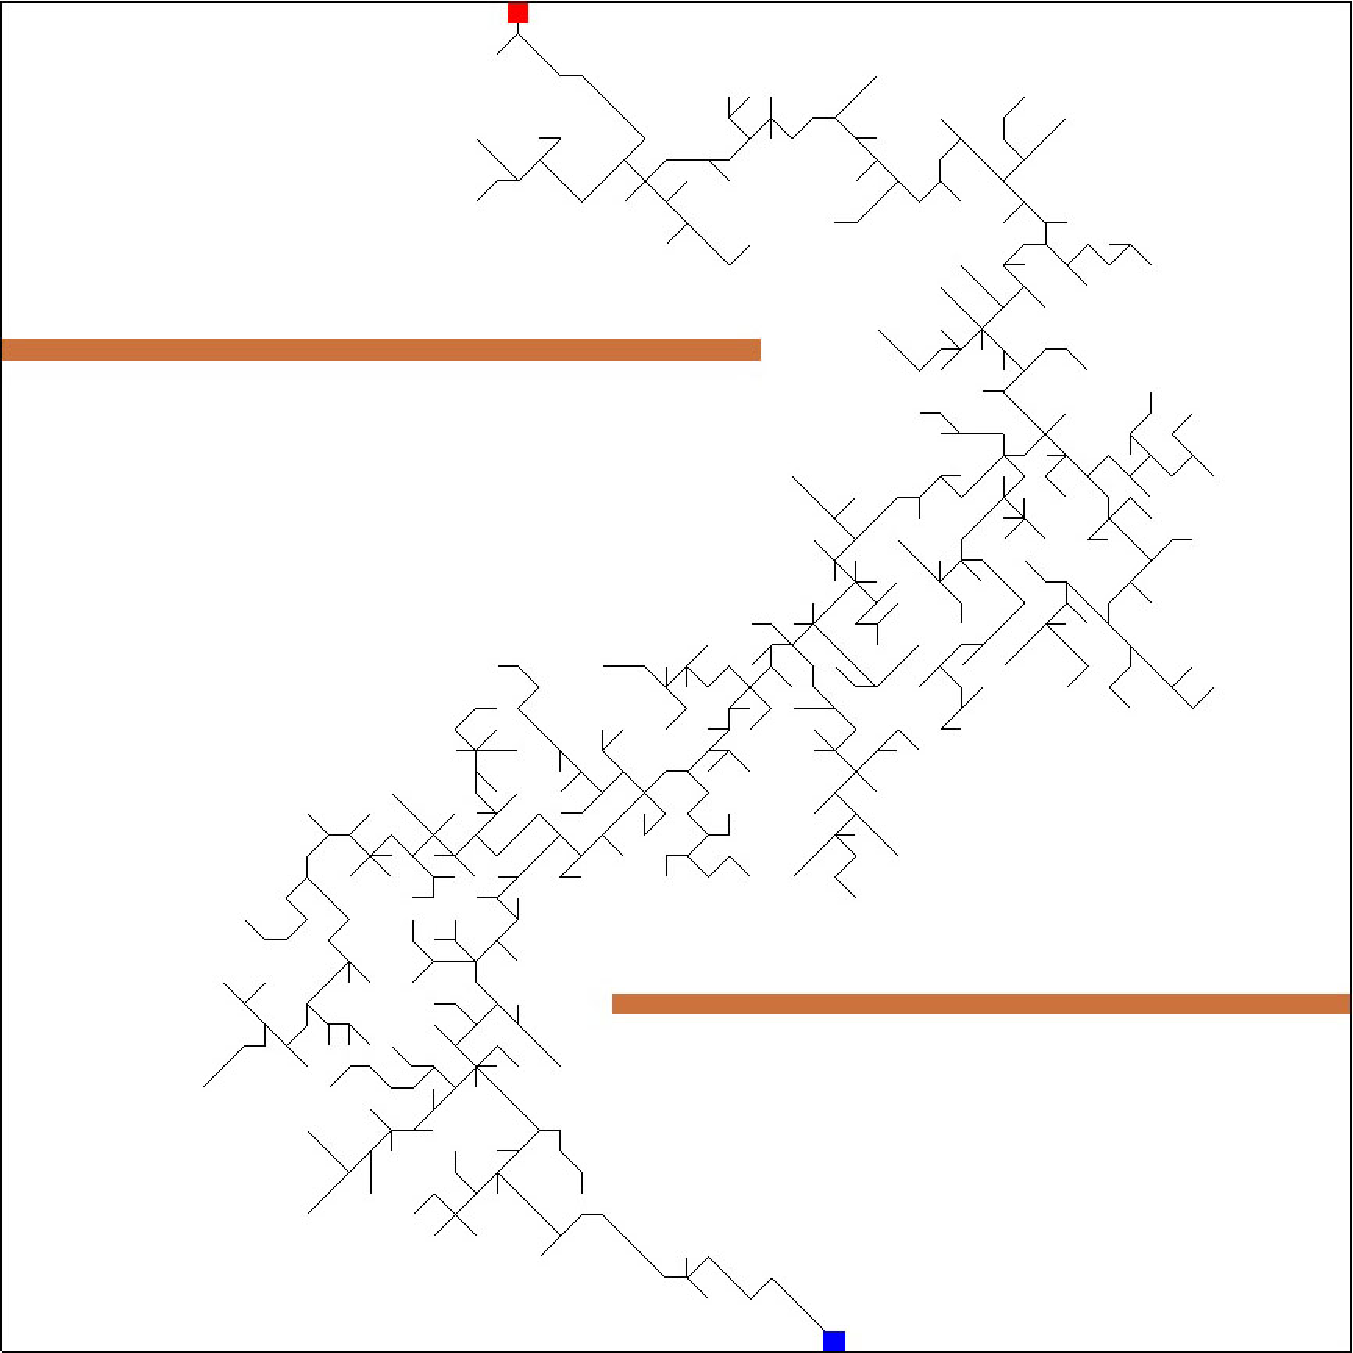
\includegraphics[width=1.6in]{fig/our_64_obs}}
	\subfigure[Result for very complex scene]{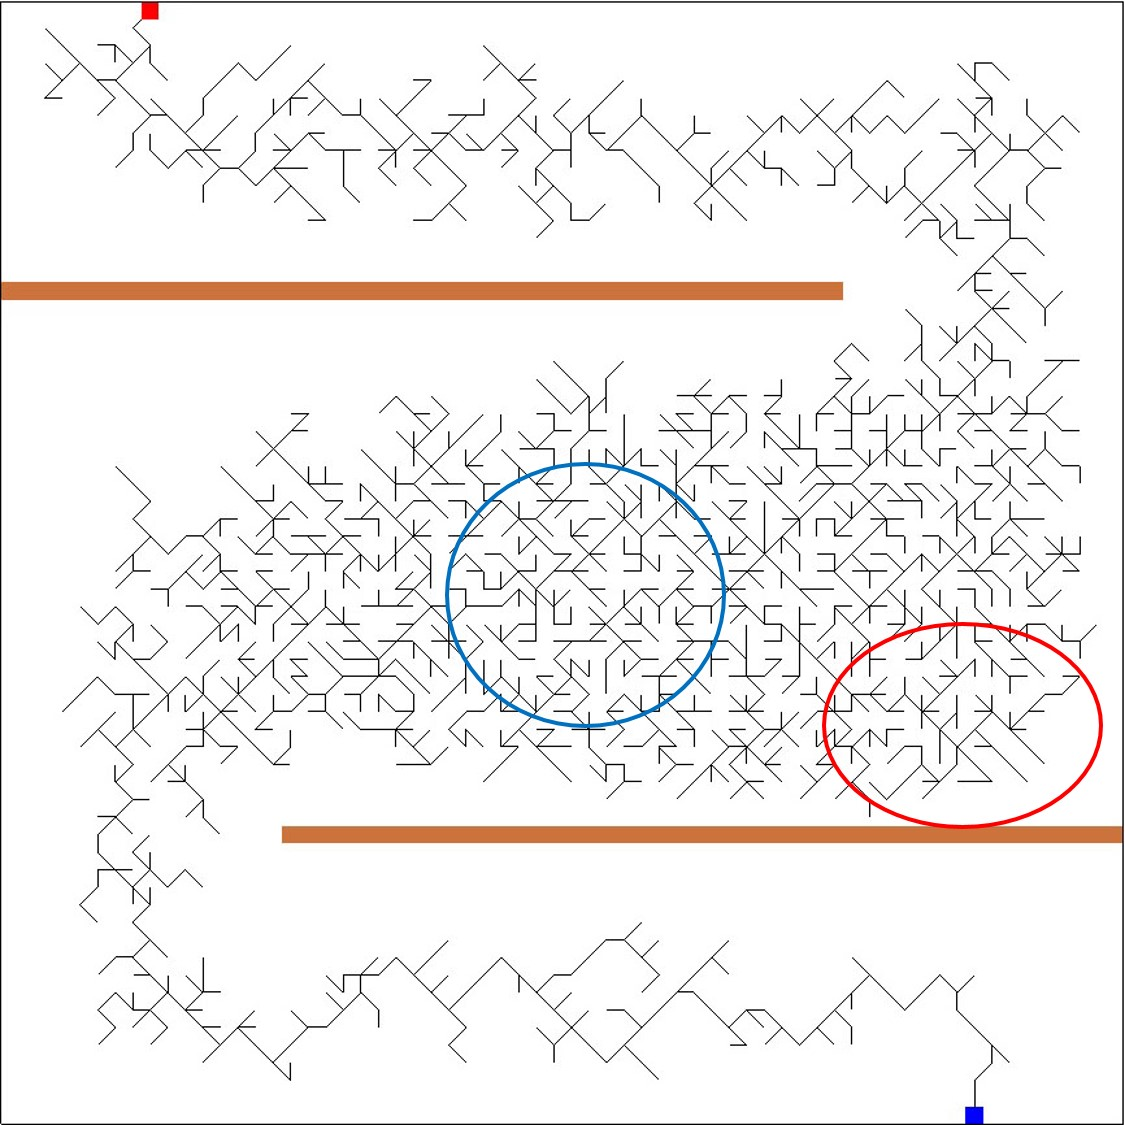
\includegraphics[width=1.6in]{fig/our_64_obs_complex}}
	\subfigure[Result for very complex scene with waypoints]{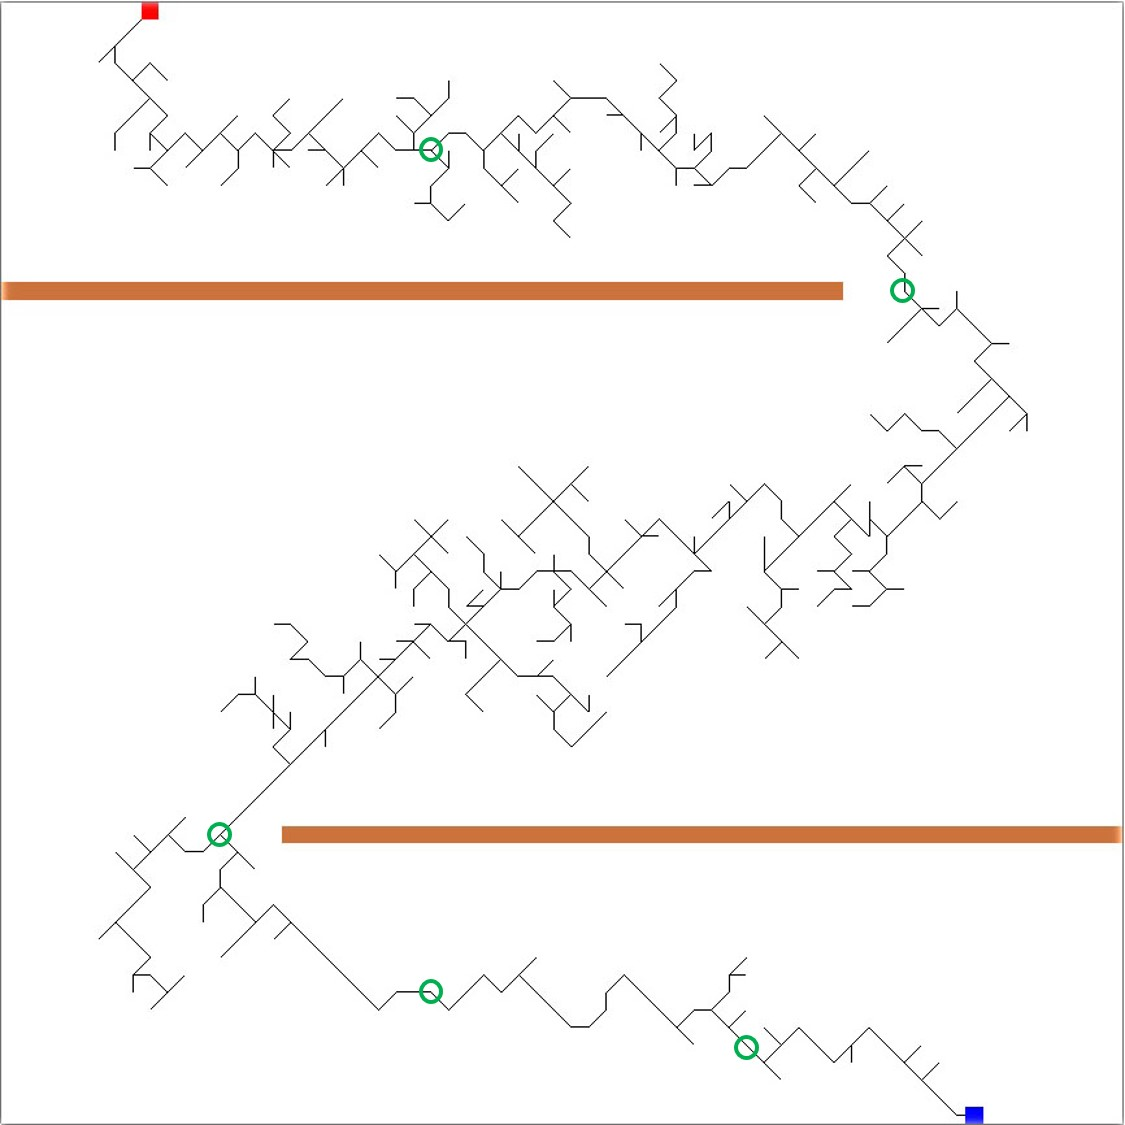
\includegraphics[width=1.6in]{fig/our_64_obs_complex_waypoints}}
	\caption{The lightning shape for complex scenes whish have obstacels. Red and blue rectangles show the starting and goal position of the lightning. The light brown objects represent obstacles what the lightning should avoid. (a) shows the lightning shape for less complex scene. (b) shows the local minima problem for very complex scene. Cells in red circle are closer to the goal than cells in blue circle even though they are not visible from the goal. (c) shows the result with waypoints that are represented by green circles.}
	\label{fig_comp_obs}
\end{figure}



\subsection{Rendering}

We utilize physical characteristics such as thickness and brightness of the lightning stream that are used by~\cite{Reed1994} and~\cite{Kim2004} to render the lightning. ~\cite{Kim2004} divides the lightning stream into the main channel and secondary channel. The main channel is a path that connects starting point and target point. The secondary channel is sub-branch from the main channel. They use a fixed intensity for the main channel. For the secondary channel, they apply reduced intensity in proportion to the distance from the main channel. ~\cite{Reed1994} utilizes an observed property that the thickness of the main channel is double for the secondary channel. 

Our rendering algorithm uses deferred rendering technique and is implemented by OpenGL Shading Language(GLSL). We render a scene and lightning to separate framebuffer texture. For rendering the lightning, we apply the thickness and brightness of branch with considering depth buffer. Lines of the lightning are rendered by using billboards technique as rectangles. To represent the glow effect of the lightning, we use fast two-pass Gaussian blur filter which is a widely used technique in games. First, we apply the Gaussian blur horizontally to the framebuffer texture of lightning and then, use the filter vertically to the previous result. At the last stage, we combine two textures to get the final image. We also utilize jittering technique~\cite{Kim2007} to reduce an artifact of grid regularities that appear due to lack of grid resolution. Figure.~\ref{fig_rendering_process} shows overall process of our rendering method.

\begin{figure}[h]
	\centering
	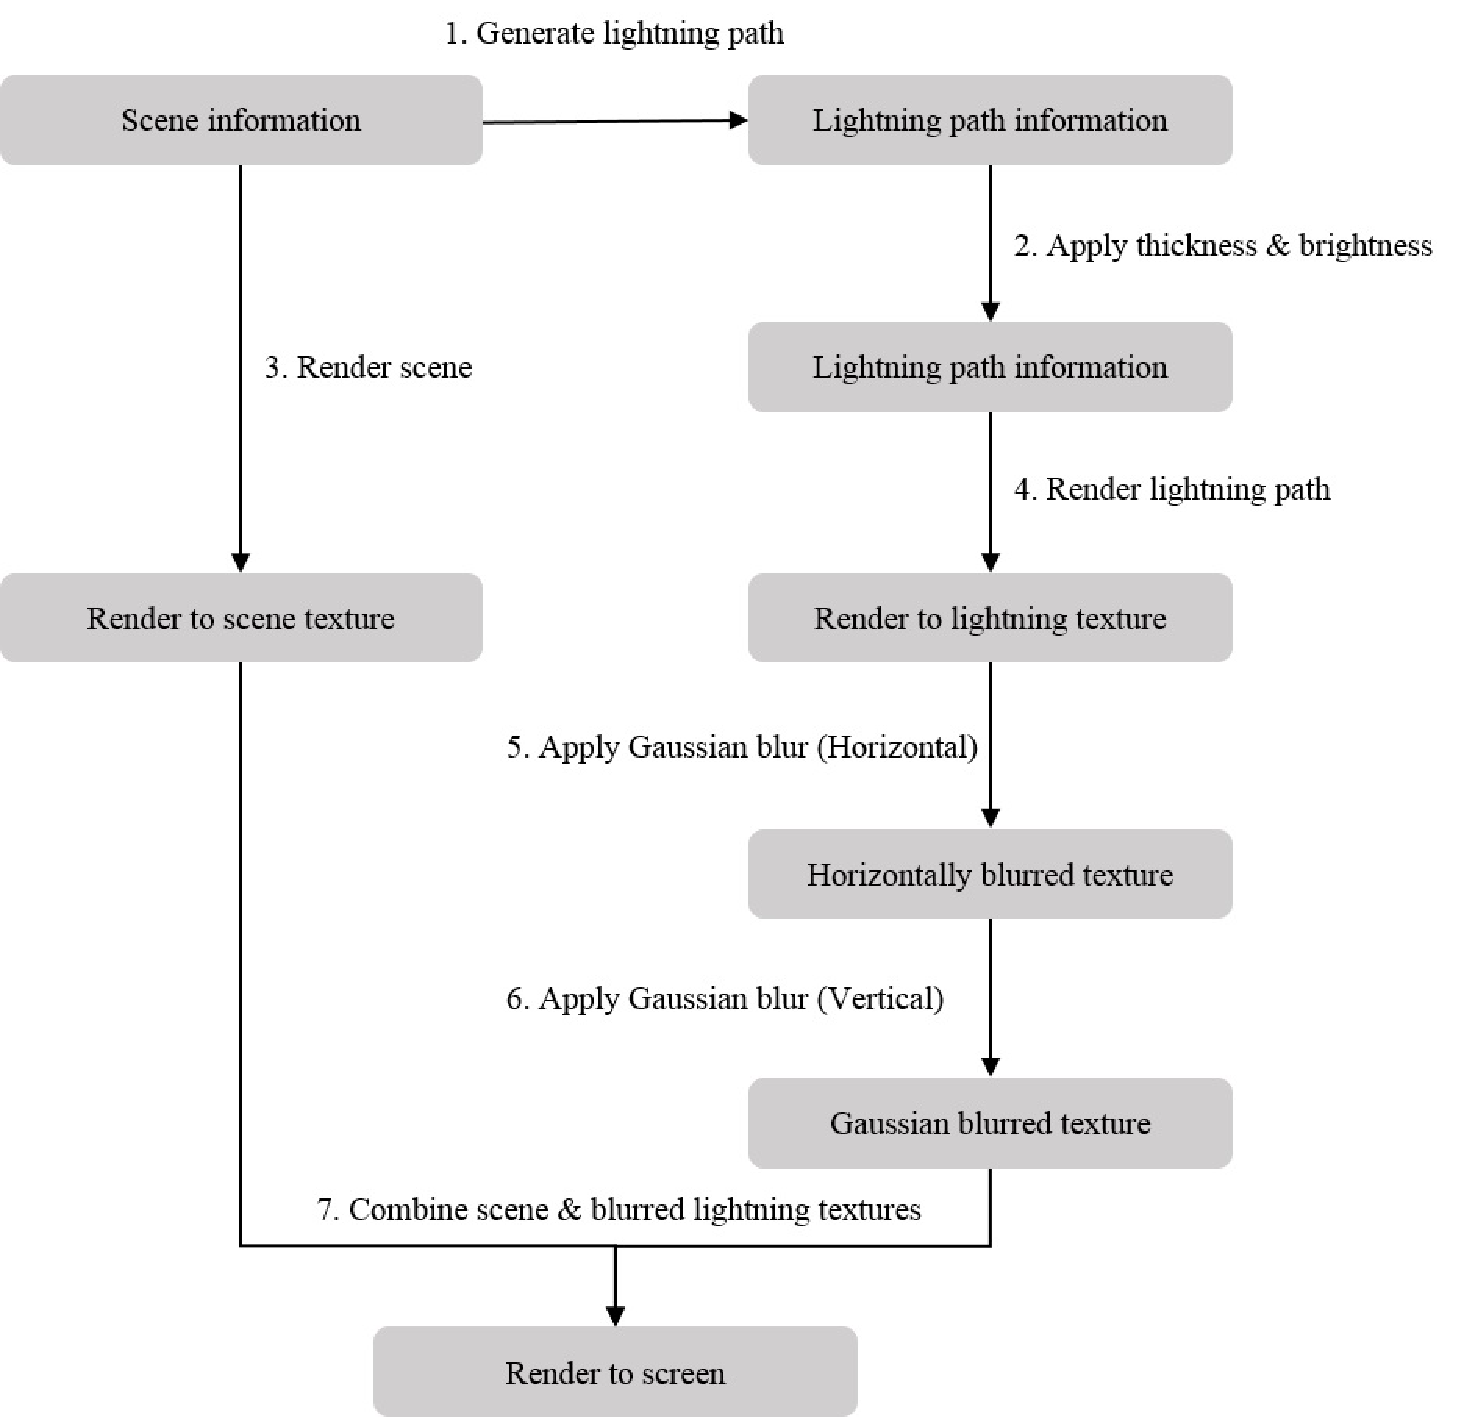
\includegraphics[width=3.0in]{fig/rendering_process}
	\caption{Overall rendering process}
	\label{fig_rendering_process}
\end{figure}

